\documentclass[11pt,a4paper]{article}

% ── Fonts & encoding ─────────────────────────────────────────────────────────
\usepackage[T1]{fontenc}
\usepackage[utf8]{inputenc}
\usepackage[sfdefault]{FiraSans}   % Inter-like sans for the whole document
\usepackage[scaled=0.85]{beramono} % clean monospace for code tokens

% ── Layout ───────────────────────────────────────────────────────────────────
\usepackage[a4paper,margin=2.3cm]{geometry}
\usepackage{enumitem}
\setlist{nosep,leftmargin=1.4em}
\usepackage{booktabs}
\usepackage{array}
\usepackage{xcolor}
\usepackage{titlesec}
\usepackage{tcolorbox}
\usepackage{tikz}
\usetikzlibrary{positioning,arrows.meta}
\usepackage{fancyhdr}

% ── FitDash "Training Copilot Professional" palette ──────────────────────────
\definecolor{fdNavy}{HTML}{0B1219}
\definecolor{fdSlate}{HTML}{16212B}
\definecolor{fdBorder}{HTML}{1E293B}
\definecolor{fdTeal}{HTML}{2DD4BF}
\definecolor{fdTealDark}{HTML}{14B8A6}
\definecolor{fdOrange}{HTML}{F97316}
\definecolor{fdMuted}{HTML}{64748B}
\definecolor{fdGreen}{HTML}{10B981}
\definecolor{fdAmber}{HTML}{F59E0B}

\usepackage[colorlinks=true,linkcolor=fdTealDark,urlcolor=fdTealDark,citecolor=fdTealDark]{hyperref}

% ── Section styling: navy bold title + teal underrule ────────────────────────
\titleformat{\section}{\large\bfseries\color{fdNavy}}{\thesection}{0.6em}{}[{\color{fdTeal}\titlerule[1.2pt]}]
\titleformat{\subsection}{\normalsize\bfseries\color{fdTealDark}}{\thesubsection}{0.5em}{}
\titlespacing*{\section}{0pt}{1.4ex}{0.8ex}
\titlespacing*{\subsection}{0pt}{1.0ex}{0.4ex}

% ── Header / footer ──────────────────────────────────────────────────────────
\pagestyle{fancy}\fancyhf{}
\renewcommand{\headrulewidth}{0pt}
\fancyfoot[L]{\footnotesize\color{fdMuted}FitDash — Training Copilot}
\fancyfoot[C]{\footnotesize\color{fdMuted}System Architecture}
\fancyfoot[R]{\footnotesize\color{fdMuted}\thepage}

% Inline code token
\newcommand{\code}[1]{{\small\texttt{#1}}}

% Layer node + flow arrow styles for the architecture figure
\tikzset{
  layer/.style={draw=fdBorder, line width=0.7pt, rounded corners=5pt,
                text width=14.2cm, align=center, inner ysep=6pt, inner xsep=6pt,
                font=\footnotesize},
  flow/.style={-{Stealth[length=2.6mm]}, line width=1.1pt, draw=fdTealDark},
}

\begin{document}

% ── Title banner ─────────────────────────────────────────────────────────────
\begin{tcolorbox}[colback=fdNavy,colframe=fdNavy,boxrule=0pt,rounded corners,
                  left=14pt,right=14pt,top=12pt,bottom=12pt]
  \color{white}{\Huge\bfseries FitDash}\\[3pt]
  {\large\color{white} Training Copilot --- System Architecture}\\[8pt]
  {\small\color{fdTeal} AISS2 \,\textbullet\, Team 6 \,\textbullet\, Karlsruhe Institute of Technology
   \hfill \today}
\end{tcolorbox}

\vspace{0.6em}

\noindent
FitDash (the \emph{Training Copilot}) is a sports-analytics assistant that unifies an
athlete's Strava activities, Garmin wearable metrics, live weather, routing and calendar
behind a single agentic chat. Its defining rule is that \textbf{every answer is grounded in
data fetched live from real tools} --- nothing is invented or cached-summarised. This
document describes the key architecture: a multi-agent chat engine layered on top of a
uniform, tool-agnostic data plane.

% ── Key idea callout ─────────────────────────────────────────────────────────
\begin{tcolorbox}[colback=fdTeal!8,colframe=fdTeal,coltitle=fdNavy,fonttitle=\bfseries,
                  title=The load-bearing idea: MCP-standard and tool-agnostic,
                  boxrule=1pt,rounded corners,left=8pt,right=8pt,top=5pt,bottom=5pt]
One uniform client talks to many independent servers; tools are \emph{discovered, never
hardcoded}; and authentication is separated from tool declarations. Adding a data source
is one new server file plus one registry line --- no change to the host, the agents, or the
UI. Internalising this explains where every component lives.
\end{tcolorbox}

% =============================================================================
\section{System overview}
% =============================================================================
The system is a vertical stack of well-separated layers. A user request enters at the top,
is decomposed by an orchestrator agent, delegated to specialist agents, and resolved against
external data through a single tool-calling seam. Two paths run through it: the \emph{chat
path} (UI $\rightarrow$ orchestrator $\rightarrow$ specialists) and the \emph{data path}
(agent $\rightarrow$ \code{ToolHost} $\rightarrow$ MCP servers $\rightarrow$ external APIs).

\begin{figure}[ht]
\centering
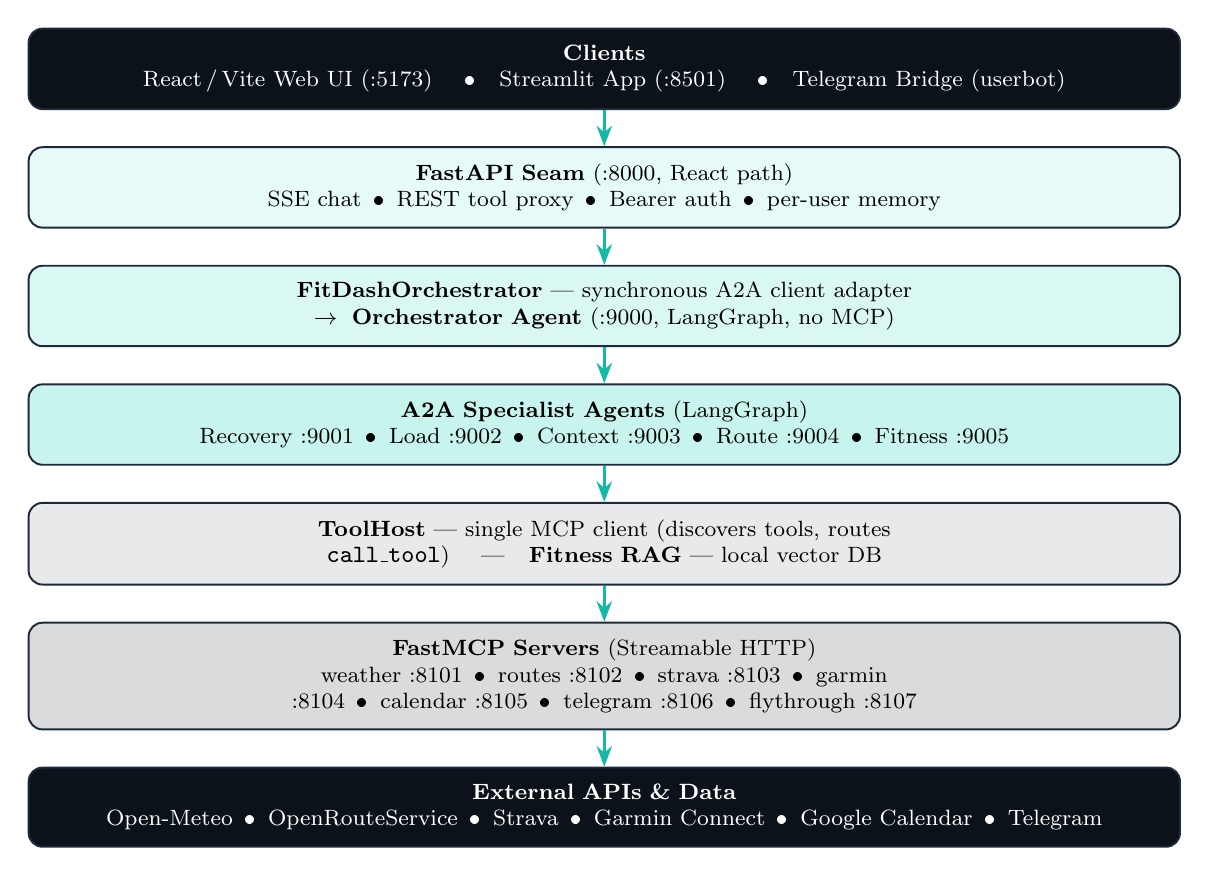
\begin{tikzpicture}[node distance=4.6mm]
  \node[layer, fill=fdNavy, text=white] (clients)
    {\textbf{Clients} \\ React\,/\,Vite Web UI (:5173) \quad\textbullet\quad
     Streamlit App (:8501) \quad\textbullet\quad Telegram Bridge (userbot)};
  \node[layer, fill=fdTeal!12, below=of clients] (api)
    {\textbf{FastAPI Seam} (:8000, React path) \\
     SSE chat \,\textbullet\, REST tool proxy \,\textbullet\, Bearer auth \,\textbullet\, per-user memory};
  \node[layer, fill=fdTeal!18, below=of api] (orch)
    {\textbf{FitDashOrchestrator} --- synchronous A2A client adapter \;$\rightarrow$\;
     \textbf{Orchestrator Agent} (:9000, LangGraph, no MCP)};
  \node[layer, fill=fdTeal!26, below=of orch] (spec)
    {\textbf{A2A Specialist Agents} (LangGraph) \\
     Recovery :9001 \,\textbullet\, Load :9002 \,\textbullet\, Context :9003 \,\textbullet\,
     Route :9004 \,\textbullet\, Fitness :9005};
  \node[layer, fill=fdSlate!10, below=of spec] (tools)
    {\textbf{ToolHost} --- single MCP client (discovers tools, routes \code{call\_tool})
     \quad|\quad \textbf{Fitness RAG} --- local vector DB};
  \node[layer, fill=fdSlate!16, below=of tools] (mcp)
    {\textbf{FastMCP Servers} (Streamable HTTP) \\
     weather :8101 \,\textbullet\, routes :8102 \,\textbullet\, strava :8103 \,\textbullet\,
     garmin :8104 \,\textbullet\, calendar :8105 \,\textbullet\, telegram :8106 \,\textbullet\, flythrough :8107};
  \node[layer, fill=fdNavy, text=white, below=of mcp] (ext)
    {\textbf{External APIs \& Data} \\ Open-Meteo \,\textbullet\, OpenRouteService \,\textbullet\,
     Strava \,\textbullet\, Garmin Connect \,\textbullet\, Google Calendar \,\textbullet\, Telegram};

  \draw[flow] (clients)--(api);
  \draw[flow] (api)--(orch);
  \draw[flow] (orch)--(spec);
  \draw[flow] (spec)--(tools);
  \draw[flow] (tools)--(mcp);
  \draw[flow] (mcp)--(ext);
\end{tikzpicture}
\caption{Layered architecture. The React UI reaches the orchestrator through the FastAPI
seam; the Streamlit app and the Telegram bridge embed \code{FitDashOrchestrator}
in-process. All upstream data access funnels through \code{ToolHost}.}
\end{figure}

% =============================================================================
\section{Core seams (\texttt{core/})}
% =============================================================================
\code{core/} is deliberately Streamlit-free and vendor-neutral, so it can run standalone
behind any front-end. Four small modules carry the architecture:

\begin{description}[style=unboxed,leftmargin=0em,itemsep=2pt]
  \item[\code{config.py} --- the registry.] A flat \code{name $\rightarrow$ URL} dictionary
    (\code{MCP\_SERVERS}) plus the A2A agent registry (\code{A2A\_AGENTS}) and the per-agent
    tool scope (\code{AGENT\_MCP\_SCOPE}). Every URL is environment-overridable. Tool names are
    namespaced \code{server\_\_tool} (the separator \code{SEP="\_\_"}, since dots are illegal in
    OpenAI function names).
  \item[\code{host.py} --- \code{ToolHost}.] The single MCP client for the entire app.
    \code{list\_tools()} discovers every tool from every \emph{reachable} server in OpenAI-tool
    format; an unreachable or unauthorised server is silently skipped, never fatal.
    \code{call\_tool("server\_\_tool", args)} splits the name, routes the call, and returns
    text/JSON --- tool errors come back as \code{\{"error": \ldots\}} strings, not exceptions.
    The implementation is async with a synchronous facade for thread/Streamlit callers.
  \item[\code{llm.py} --- the LLM seam.] The only place a chat client is constructed and the
    model resolved, both from \code{.env}. \code{LLM\_PROVIDER} switches the whole app between
    \code{openai} (KIT gateway or any OpenAI-compatible endpoint), \code{openai\_official}
    (api.openai.com), and \code{gemini} --- a configuration change, not a code change. The seam
    re-reads \code{.env} per call, so a model switch in the Settings UI applies without restart.
  \item[\code{orchestrator.py} --- \code{FitDashOrchestrator}.] A thin synchronous \emph{A2A
    client adapter} to the orchestrator agent. It preserves one stable public contract for all
    callers --- \code{run(user\_input, history, progress\_cb, text\_cb) $\rightarrow$ (answer,
    trace)} and \code{refresh\_tools()} --- so the React seam, the Streamlit chat, and the
    Telegram bridge are interchangeable front-ends over the same engine.
\end{description}

% =============================================================================
\section{Agent layer --- LangGraph specialists over A2A}
% =============================================================================
The chat engine is a multi-agent system. Each agent is its own \textbf{A2A server} (the
official \code{a2a-sdk}, exposing an Agent Card at \code{/.well-known/agent-card.json}), so
agents are independently deployable and discoverable.

\paragraph{Orchestrator (:9000).} A LangGraph agent whose only tools are \code{ask\_*} ---
one per specialist, each performing an A2A call. It decomposes the user request, delegates
(in \emph{parallel} when the model emits several tool calls at once), collects each
specialist's \code{DataPart} artifact, and assembles the structured \code{trace} via
\code{core/agent\_trace.build\_trace}. It has \textbf{no MCP access} of its own --- it only
coordinates.

\paragraph{Specialists.} Each is a LangGraph ReAct agent over a \code{ToolHost} scoped to a
narrow set of MCP servers. Tools remain discovered, never hardcoded --- merely narrowed per
agent. Specialists return their raw MCP results (full JSON) as artifacts so the orchestrator
can build route maps, charts, and the debug trace.

\begin{table}[ht]\centering\footnotesize
\renewcommand{\arraystretch}{1.25}
\begin{tabular}{@{}>{\bfseries}l c l p{7.4cm}@{}}
\toprule
\normalfont\textbf{Agent} & \textbf{Port} & \textbf{MCP scope} & \textbf{Responsibility} \\
\midrule
Orchestrator & 9000 & --- & Decompose request, delegate in parallel, synthesise answer, build trace \\
Recovery     & 9001 & garmin & Sleep, HRV, Body Battery, stress $\rightarrow$ readiness / should I rest? \\
Load         & 9002 & strava, garmin & Training load \& trends (CTL/ATL/TSB), PBs, pace, HR zones, activity detail \\
Context      & 9003 & weather, calendar & Weather forecast $\times$ calendar free time $\rightarrow$ best training window; writes calendar events \\
Route        & 9004 & routes & Plan routes / loops / park loops / trails, geocode places, elevation, isochrones \\
Fitness      & 9005 & --- (RAG) & Training methods \& technique answered from a vector DB of fitness literature, with citations \\
\bottomrule
\end{tabular}
\caption{The orchestrator and the five specialists. Scope comes from \code{AGENT\_MCP\_SCOPE};
unreachable specialists degrade gracefully rather than failing the turn.}
\end{table}

\paragraph{Fitness Expert --- the RAG exception.} The fitness agent has no MCP server. It
answers exercise-science questions from a local vector database of public-domain fitness
books (\code{core/fitness\_rag.py}). Its single \code{search\_fitness\_literature} tool is
recorded in the same artifact shape as any MCP call, so it flows into the trace uniformly.
Embeddings use a small \emph{local} model (\code{sentence-transformers}, all-MiniLM-L6-v2)
--- no embedding API.

% =============================================================================
\section{Data plane --- MCP servers \& integrations}
% =============================================================================
Each data source is a self-contained \textbf{FastMCP} server over Streamable HTTP. There is
no shared base class and no dispatch indirection: a tool calls its upstream API directly and
returns clean JSON. The \code{@mcp.tool()} docstring \emph{is} the tool's interface --- it is
what the model reads to choose a tool.

\begin{table}[ht]\centering\footnotesize
\renewcommand{\arraystretch}{1.25}
\begin{tabular}{@{}>{\bfseries}l c l@{}}
\toprule
\normalfont\textbf{Server} & \textbf{Port} & \textbf{Upstream / role} \\
\midrule
weather    & 8101 & Open-Meteo --- forecast, current conditions, UV, pollen \\
routes     & 8102 & OpenRouteService --- routing, circular \& park loops, trails, elevation, isochrones \\
strava     & 8103 & Strava --- activities, training trends, personal bests, streams \\
garmin     & 8104 & Garmin Connect --- sleep, HRV, Body Battery, stress, training metrics \\
calendar   & 8105 & Google Calendar --- read and write events \\
telegram   & 8106 & \emph{Proxy} bridging the external \code{chigwell/telegram-mcp} (stdio $\rightarrow$ HTTP) \\
flythrough & 8107 & 3D GPS-track flythrough render support \\
\bottomrule
\end{tabular}
\caption{The MCP server registry (\code{MCP\_SERVERS}). Credentials are passed as connection
headers via \code{ToolHost(headers=\ldots)} --- never as tool arguments, never in model context.}
\end{table}

The \textbf{Telegram} server is the one proxy rather than a native server: it runs the
upstream stdio-only MCP project unmodified in an isolated environment and re-exposes its
tools on the Streamable-HTTP bus, holding one persistent upstream session. To \code{ToolHost}
it looks identical to every other server --- the template for bridging any external stdio MCP
server into the app.

% =============================================================================
\section{Request lifecycle}
% =============================================================================
\begin{enumerate}[label=\textbf{\arabic*.}]
  \item A user asks a question in the React chat, the Streamlit app, or over Telegram. The
        client calls \code{FitDashOrchestrator.run(question, history)} --- in-process
        (Streamlit, Telegram) or through the FastAPI SSE endpoint (React).
  \item \code{run()} flattens the history into one A2A message and sends it to the
        Orchestrator Agent (:9000).
  \item The orchestrator (LangGraph) decomposes the request and invokes one or more
        \code{ask\_*} tools --- each an A2A call to a specialist --- \emph{in parallel} when the
        sub-questions are independent.
  \item Each specialist discovers the tools of its scoped MCP servers via \code{ToolHost} and
        calls the ones it needs (the Fitness agent retrieves from its RAG store instead). All
        upstream access goes through \code{call\_tool}; failures return an \code{\{"error"\}}
        payload rather than throwing.
  \item Specialists return raw results as A2A \code{DataPart} artifacts. The orchestrator
        synthesises the final answer and assembles a structured \code{trace} (tool calls,
        agents, route data, timings).
  \item The answer streams back to the client; the UI renders inline route maps and charts
        from the trace. Every agent run is traced to MLflow (Section~\ref{sec:obs}).
\end{enumerate}

% =============================================================================
\section{Observability --- MLflow tracing}\label{sec:obs}
% =============================================================================
Every agent run is traced to an MLflow tracking server (UI on :5001). \code{core/tracing.py}
is the seam: each agent process enables \code{mlflow.langchain.autolog()} once and wraps its
invocation in a labelled root span tagged with its \code{service} (orchestrator / recovery /
load / context / route). The autologged LLM and tool spans nest beneath that root, so one
tagged trace per run lands in the shared \code{fitdash} experiment --- filterable by service,
with each \code{ask\_*} delegation and each MCP tool call as a child span. Tracing is
best-effort: a missing or unreachable MLflow server logs once and is ignored, and the agents
run untraced.

% =============================================================================
\section{Clients, entry points \& cross-cutting concerns}
% =============================================================================
\begin{description}[style=unboxed,leftmargin=0em,itemsep=2pt]
  \item[React / Vite web app (\code{web/}).] The primary UI (Dashboard, Health, Routes,
    Analysis, Chat, Sync, Settings). It reaches the engine through the \textbf{FastAPI seam}
    (\code{api/}), which exposes SSE chat, a REST tool proxy, settings, sync, and memory.
  \item[Streamlit app (\code{app.py}).] The legacy UI, embedding \code{FitDashOrchestrator}
    directly in-process.
  \item[Telegram bridge (\code{telegram\_bridge.py}).] A userbot that forwards each message
    (and locally transcribed voice memos) to the same orchestrator and returns the answer,
    delivering routes as a static map, a Google Maps link, and a GPX file.
  \item[Identity \& auth.] The FastAPI seam authenticates with stateless HMAC Bearer tokens
    (\code{api/auth.py}); protected routers depend on the current user.
  \item[Per-user memory.] Each user has a self-updating ``soul'' profile (Markdown the agent
    periodically distils from the conversation) plus a per-user conversation vector store for
    exact recall (all-MiniLM-L6-v2), blended into the orchestrator prompt.
\end{description}

% =============================================================================
\section{Extensibility \& technology stack}
% =============================================================================
The architecture optimises for one operation: \textbf{adding a data source}. Write a FastMCP
server file with \code{@mcp.tool()} functions, add one line to \code{MCP\_SERVERS}, start the
process --- and the chat agents can call it immediately. No change to the host, orchestrator,
or UI. Adding a \emph{specialist} is symmetric: one A2A agent process plus one registry entry.

\begin{table}[ht]\centering\footnotesize
\renewcommand{\arraystretch}{1.25}
\begin{tabular}{@{}>{\bfseries}l l@{}}
\toprule
\normalfont\textbf{Layer} & \textbf{Technology} \\
\midrule
LLM seam        & LangChain \code{ChatOpenAI} / Gemini; provider via \code{LLM\_PROVIDER} \\
Agents          & LangGraph (\code{create\_agent} / ReAct) over \code{a2a-sdk} (A2A protocol, agent cards) \\
Tools / data    & MCP --- FastMCP servers (Streamable HTTP) behind a single \code{ToolHost} \\
Web front-end   & React + Vite + TypeScript + Tailwind (\code{web/}); FastAPI seam (\code{api/}) \\
Legacy UI       & Streamlit (\code{app.py}) \\
Messaging       & Telethon userbot (\code{telegram\_bridge.py}) \\
RAG             & \code{sentence-transformers} all-MiniLM-L6-v2 + local NumPy vector store \\
Observability   & MLflow tracing (autolog + tagged spans) \\
\bottomrule
\end{tabular}
\caption{Technology stack by architectural layer.}
\end{table}

\end{document}
